\documentclass{article}
\usepackage[utf8]{inputenc}
\parskip = 0.75em
\parindent = 10mm
\def\baselinestretch{1}
\usepackage {float}
\usepackage{listings}
\usepackage[usenames]{color}
\usepackage[numbers,sort&compress]{natbib}
\usepackage{multirow, array}
\usepackage[spanish]{babel}
	\deactivatetilden
	\spanishdecimal{.}
	\addto\captionsspanish{\def\tablename{Tabla}}
	\addto\captionsspanish{\def\listtablename{\'Indice de tablas}}

\usepackage{amsmath,amsfonts,amssymb}
	\allowdisplaybreaks[4]
\usepackage{graphicx}
	\graphicspath{{Figuras/}}
\usepackage[clearempty,pagestyles]{titlesec}
\usepackage{anysize}

\def\baselinestretch{1.5}
\papersize{27.9cm}{21.5cm} 
\marginsize{2cm}{2cm}{1cm}{1cm}

\begin{document}


	\begin{center}
	\huge{\textbf{Tarea 2 Simulación del Juego de la Vida (Autómata Celular)}}
	\line(1,0) {300}\\
	
	\textsc{ \Large Susana Ruiz Nuñez} 
	\textsc{ \Large 2032426}
	\end{center}


\section{Planteamiento del Problema} 
Se requiere simular un autómata celular en dos dimensiones, particularmente el juego de la vida \cite{satu}. El estado del autómata se representa con una matríz booleana. Cada celda está viva si su valor es uno o muerta si es cero. En cada paso, la supervivencia de cada celda se determina a partir de los valores de sus ocho vecinos, (no se considera así en los extremos). La regla de supervivencia es sencilla: una celda está viva si exactamente tres vecinos suyos están vivos. 

\section{Metodología}
Para comenzar, se creó un for para generar números aleatorios cuya aleatoriedad estuviera condicionada por una probabilidad inicial, ya que en esto constituía la orden para esta práctica, en poder variar la probabilidad inicial de celda viva para valores entre 0.1 y 0.9. Para esto en Python se utilizan los paquetes numpy y el matplotlib. 
  
\begin{lstlisting}[language=Python]
	for i in range(orden):
	generacionNumeros = random()
		if generacionNumeros < probabilidadVivir:
		values[i] = 1
			else:
		values[i] = 0
\end{lstlisting}

A continuación se creó el Juego de la Vida \cite{satu} con la condición de que se detuviera al morir todas las celdas y en el caso de que no, al llegar a un máximo de 50 iteraciones (para Python 49 iteraciones). Para cada iteración se guardan el número de vivos y se agregó una condición para calcular el colapso mayor. 
\begin{lstlisting}[language=Python]
	for iteracion in range(49):
		values = [gameOfLife(x) for x in range(orden)]
		colapso = vivosActual - vivos
		vivosActual = vivos
		if colapso > colapsoMayor:
			colapsoMayor = colapso
\end{lstlisting}
     
\section{Resultados}
Como se muestra en la (Figura 1) ninguna prueba rebasó la iteración 11 del total de 50 a las que podían llegar. Mientras mayor es la probabilidad inicial de celda viva, mayor número de vivos se tienen en la matriz inicial (iteración 0), pero a su vez el colapso es mayor entre iteraciones consecutivas y muere más rapidamente, es decir, en tan solo las primeras iteraciones llega a 0 el número de celdas vivas. 

\begin{figure}[H]
    \centering

    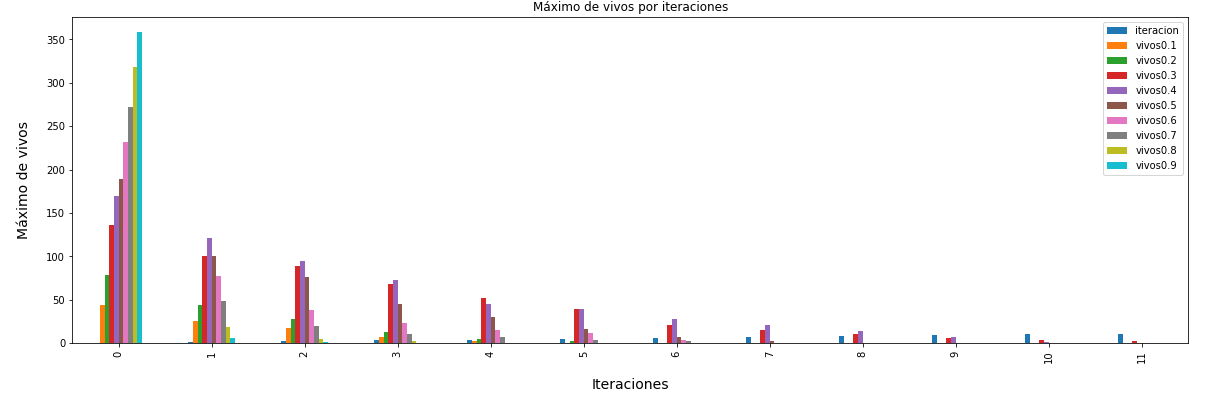
\includegraphics[scale=0.6]{Captura1.png}
    \caption{Número máximo de vivos por iteraciones}
    \label{fig:f1}
\end{figure}


A continuación se muestran de los datos recopilados, un cuadro indicando el  mayor colapso ocurrido entre iteraciones consecutivas. Como se muestra en la información los grandes saltos fueron dados todos de la matriz inicial a la primera iteración.
\begin{center}
\begin{tabular}{|c|c|c|c|}
\hline 
Probabilidad & Máximo colapso & Iteración \\ 
\hline 
0.1 & 19 & Iteración 1 \\ 
\hline 
0.2 & 34 & Iteración 1 \\ 
\hline 
0.3 & 36 & Iteración 1 \\ 
\hline 
0.4 & 48 & Iteración 1 \\ 
\hline 
0.5 & 89 & Iteración 1 \\ 
\hline 
0.6 & 155 & Iteración 1 \\ 
\hline 
0.7 & 224 & Iteración 1 \\ 
\hline 
0.8 & 299 & Iteración 1 \\
\hline 
0.9 & 352 & Iteración 1 \\ 
\hline
\end{tabular}
\end{center}
\begin{center}
	Tabla 1: Máximo colapso por probabilidad de celda viva
\end{center}

Se realizó un análisis también para observar el comportamiento entre iteraciones consecutivas para cada probabibilidad inicial de celda viva. Se muestra en la (Figura 2) como para las probabilidades más pequeñas el colapso es más uniforme, mientras que para las probabilidades mayores (Figura 3)  se tiene un colapso muy grande para las primeras iteraciones y muere rápidamente. 

\begin{figure}[H]
	\centering
	
	\includegraphics[scale=0.5]{captura2.png}
	\caption{Colapso para probabibilidad inicial de celda viva de 0.1, 0.2, 0.3}
	\label{fig:f2}
\end{figure}

\begin{figure}[H]
	\centering
	
	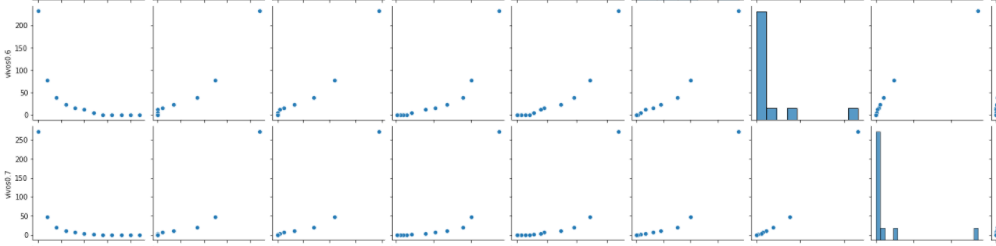
\includegraphics[scale=0.5]{Captura3.png}
	\caption{Colapso para probabibilidad inicial de celda viva de 0.6, 0.7}
	\label{fig:f3}
\end{figure}
 
\section{Conclusiones}
Se puede concluir con los experimentos realizados que al aumentar la probabilidad inicial de celda viva se logra un mayor número de vivos en la iteración inicial, pero la misma decae más rápidamente, es decir, tiene un colapso mayor que para probabilidades menores que resisten más iteraciones. 

\bibliography{Tarea2}
\bibliographystyle{plainnat}
\end{document} 
